%%===========================================================%%
%%                                                           %%
%%                     RpEfficiencySystematicsAppendix                  %%
%%                                                           %%
%%===========================================================%%

\chapter{RP track reconstruction efficiency comparison between data and MC}\label{appendix:rpTrackRecoEffSyst}

%---------------------------
\begin{figure}[h]%\vspace{-34pt}
	\centering
	\parbox{0.54\textwidth}{
		\centering
		\begin{subfigure}[b]{\linewidth}{
				\subcaptionbox{\label{fig:totalRpRecoEff2D_ED}}{\includegraphics[width=\linewidth,page=2]{graphics/systematicsEfficiency/RpSyst/totalRpRecoEff2D.pdf}\vspace{-12pt}}}
		\end{subfigure}
		\caption[Coparison of estimated RP track reconstruction efficiency in 2D and 1D (branch ED).]%
		{Comparison of RP track reconstruction efficiency in branch ED estimated with the method described in Sec.~\ref{subsec:rpTrackRecoEffSyst} as a function of $(p_{x},p_{y})$ of proton (\ref{fig:totalRpRecoEff2D_ED}) and comparison of 1-dimensional projections of efficiencies in a fiducial region marked with green envelope: $p_{x}$ (\ref{fig:totalRpRecoEff1D_ED_px}) and $p_{y}$ (\ref{fig:totalRpRecoEff1D_ED_py}). Lower pad in each subfigure shows the difference between efficiency extracted from the data and elastic scattering MC embedded into zero-bias data.}\label{fig:totalRpRecoEff_ED}\vspace{52pt}%
	}
	\quad
	\parbox{0.43\textwidth}{
		\centering
		\begin{subfigure}[b]{\linewidth}{
				\subcaptionbox{\label{fig:totalRpRecoEff1D_ED_px}}{\includegraphics[width=\linewidth,page=3]{graphics/systematicsEfficiency/RpSyst/dataTotalEff_1D.pdf}\vspace{-12pt}}}
		\end{subfigure}
		\begin{subfigure}[b]{\linewidth}{
				\subcaptionbox{\label{fig:totalRpRecoEff1D_ED_py}}{\includegraphics[width=\linewidth,page=4]{graphics/systematicsEfficiency/RpSyst/dataTotalEff_1D.pdf}\vspace{-12pt}}}
		\end{subfigure}
	}
\end{figure}
%---------------------------


%---------------------------
\begin{figure}[h]%\vspace{-34pt}
	\centering
	\parbox{0.54\textwidth}{
		\centering
		\begin{subfigure}[b]{\linewidth}{
				\subcaptionbox{\label{fig:totalRpRecoEff2D_WU}}{\includegraphics[width=\linewidth,page=3]{graphics/systematicsEfficiency/RpSyst/totalRpRecoEff2D.pdf}\vspace{-12pt}}}
		\end{subfigure}
		\caption[Coparison of estimated RP track reconstruction efficiency in 2D and 1D (branch WU).]%
		{Comparison of RP track reconstruction efficiency in branch ED estimated with the method described in Sec.~\ref{subsec:rpTrackRecoEffSyst} as a function of $(p_{x},p_{y})$ of proton (\ref{fig:totalRpRecoEff2D_WU}) and comparison of 1-dimensional projections of efficiencies in a fiducial region marked with green envelope: $p_{x}$ (\ref{fig:totalRpRecoEff1D_WU_px}) and $p_{y}$ (\ref{fig:totalRpRecoEff1D_WU_py}). Lower pad in each subfigure shows the difference between efficiency extracted from the data and elastic scattering MC embedded into zero-bias data.}\label{fig:totalRpRecoEff_WU}\vspace{52pt}%
	}
	\quad
	\parbox{0.43\textwidth}{
		\centering
		\begin{subfigure}[b]{\linewidth}{
				\subcaptionbox{\label{fig:totalRpRecoEff1D_WU_px}}{\includegraphics[width=\linewidth,page=5]{graphics/systematicsEfficiency/RpSyst/dataTotalEff_1D.pdf}\vspace{-12pt}}}
		\end{subfigure}
		\begin{subfigure}[b]{\linewidth}{
				\subcaptionbox{\label{fig:totalRpRecoEff1D_WU_py}}{\includegraphics[width=\linewidth,page=6]{graphics/systematicsEfficiency/RpSyst/dataTotalEff_1D.pdf}\vspace{-12pt}}}
		\end{subfigure}
	}
\end{figure}
%---------------------------


%---------------------------
\begin{figure}[h]%\vspace{-100pt}
	\centering
	\parbox{0.54\textwidth}{
		\centering
		\begin{subfigure}[b]{\linewidth}{
				\subcaptionbox{\label{fig:totalRpRecoEff2D_WD}}{\includegraphics[width=\linewidth,page=4]{graphics/systematicsEfficiency/RpSyst/totalRpRecoEff2D.pdf}\vspace{-12pt}}}
		\end{subfigure}
		\caption[Coparison of estimated RP track reconstruction efficiency in 2D and 1D (branch WD).]%
		{Comparison of RP track reconstruction efficiency in branch ED estimated with the method described in Sec.~\ref{subsec:rpTrackRecoEffSyst} as a function of $(p_{x},p_{y})$ of proton (\ref{fig:totalRpRecoEff2D_WD}) and comparison of 1-dimensional projections of efficiencies in a fiducial region marked with green envelope: $p_{x}$ (\ref{fig:totalRpRecoEff1D_WD_px}) and $p_{y}$ (\ref{fig:totalRpRecoEff1D_WD_py}). Lower pad in each subfigure shows the difference between efficiency extracted from the data and elastic scattering MC embedded into zero-bias data.}\label{fig:totalRpRecoEff_WD}\vspace{52pt}%
	}
	\quad
	\parbox{0.43\textwidth}{
		\centering
		\begin{subfigure}[b]{\linewidth}{
				\subcaptionbox{\label{fig:totalRpRecoEff1D_WD_px}}{\includegraphics[width=\linewidth,page=7]{graphics/systematicsEfficiency/RpSyst/dataTotalEff_1D.pdf}\vspace{-12pt}}}
		\end{subfigure}
		\begin{subfigure}[b]{\linewidth}{
				\subcaptionbox{\label{fig:totalRpRecoEff1D_WD_py}}{\includegraphics[width=\linewidth,page=8]{graphics/systematicsEfficiency/RpSyst/dataTotalEff_1D.pdf}\vspace{-12pt}}}
		\end{subfigure}
	}
\end{figure}
%---------------------------



